
%! program = pdflatex

\documentclass[12pt]{article}
\usepackage{amsmath}
\usepackage{natbib}
\usepackage{graphicx}
\usepackage{amssymb}
\usepackage{epstopdf}
\usepackage{float} % to keep the figures in place

\usepackage{color}
\newcommand{\cred}{ \color{red}}
\newcommand{\cgreen}{\color{green}}
\newcommand{\cblue}{\color{blue}}
\newcommand{\cmag}{\color{magenta}}
\newcommand{\bn}{\begin{enumerate}}
\newcommand{\en}{\end{enumerate}}
\newcommand{\bi}{\begin{itemize}}
\newcommand{\ei}{\end{itemize}}
\newcommand{\be}{\begin{eqnarray}}
\newcommand{\ee}{\end{eqnarray}}
\newcommand{\by}{\begin{eqnarray*}}
\newcommand{\ey}{\end{eqnarray*}}
\renewcommand{\labelenumi}{(\alph{enumi}) }
%
\usepackage[margin=2.2cm, includehead]{geometry}% see geometry.pdf on how to lay out the page. There's lots.
\geometry{letterpaper} % or letter or a5paper or ... etc
% \geometry{landscape} % rotated page geometry
%\bibpunct{(}{)}{;}{a}{,}{,}
%\setlength{\textwidth}{16cm}
%\setlength{\textheight}{21cm}
\def\nonumber{\global\@eqnswfalse}
\newcounter{parnum}
\newcommand{\N}{%
  \noindent\refstepcounter{parnum}%
   \makebox[\parindent][l]{\textbf{[\arabic{parnum}]}}\quad  }
% Use a generous paragraph indent so numbers can be fit inside the
% indentation space.
\setlength{\parindent}{1.5em}

% See the ``Article customise'' template for come common customisations

\date{}
%\date{} % delete this line to display the current date

%%% BEGIN DOCUMENT
\usepackage{Sweave}
\begin{document}
\Sconcordance{concordance:HW5.tex:HW5.Rnw:%
1 47 1 1 0 20 1 1 3 2 0 1 2 1 0 1 1 1 2 1 0 1 2 1 0 1 1 4 0 1 2 3 1 1 3 %
2 0 1 2 1 0 2 1 1 2 1 0 1 1 8 0 1 2 3 1 1 3 2 0 1 2 1 0 1 2 5 0 1 2 2 1 %
1 3 2 0 3 1 7 0 1 2 2 1 1 3 2 0 1 2 1 0 1 2 1 0 1 2 5 0 1 2 3 1 1 3 2 0 %
1 1 1 3 2 0 1 1 6 0 1 2 1 1 1 3 2 0 1 3 2 0 1 1 6 0 1 2 1 1 1 2 1 0 1 1 %
7 0 1 2 1 1}

%\large
%\maketitle
\newtheorem{thm}{Theorem}[section]
\newtheorem{cor}[thm]{Corollary}
\newtheorem{lem}[thm]{Lemma}
\newtheorem{prop}[thm]{Proposition}
\newtheorem{defn}[thm]{Definition}
\newtheorem{exam}[thm]{Example}
\newtheorem{qstn}[thm]{Question}

%%%
\newpage
\begin{center}
{\bf Homework 5 - STAT 511}\\
Amal Agarwal
\end{center}
%==========================
\section*{Answer 5}
\begin{figure}[H]
\begin{Schunk}
\begin{Sinput}
> # extracting the cars dataset
> data(cars)
> # response (speed) and predictor (distance) vectors
> speed<-cars$speed
> distance<-cars$dist
> # fitting the simple linear model
> fit=lm(distance~speed)
> # scatter plot with fitted line
> plot(speed,distance)
> abline(fit)
\end{Sinput}
\end{Schunk}
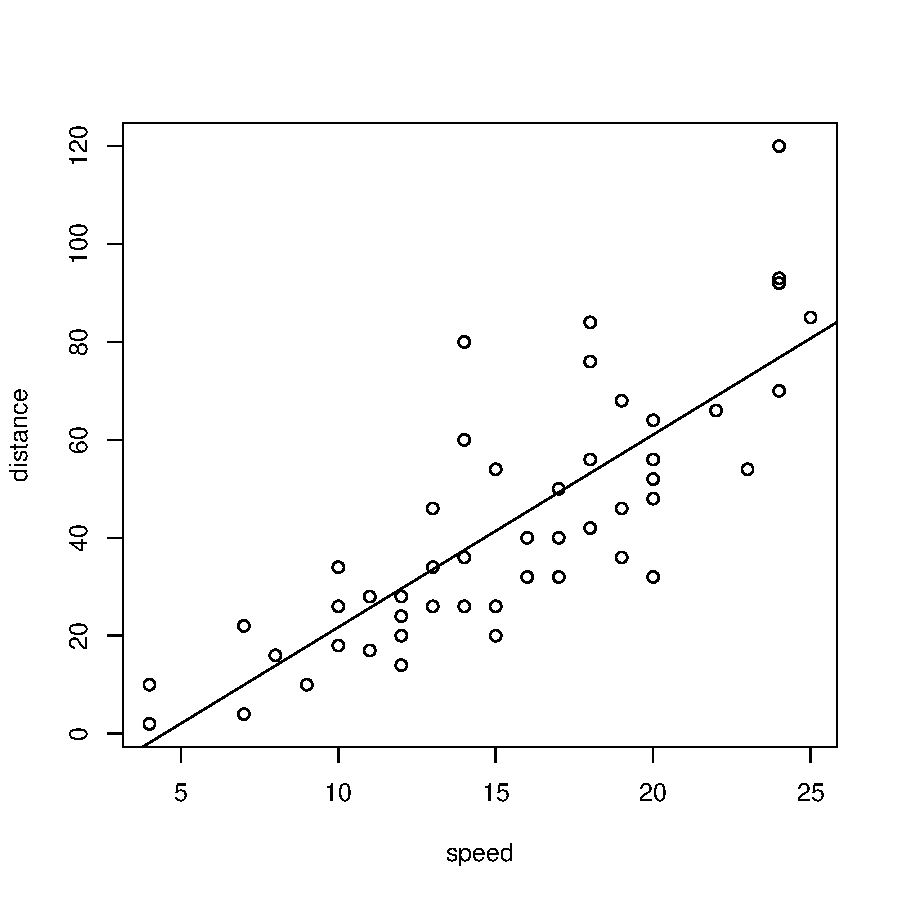
\includegraphics{HW5-001}
\end{figure}
\clearpage
\bn
\item $\hat{\beta}$ is given as
\begin{Schunk}
\begin{Sinput}
> # creating vector of 1's for intercept
> x1<-rep(1,length(speed))
> # creating design matrix
> X=matrix(0,nrow=length(speed), ncol=2)
> X[,1]<-x1
> X[,2]<-speed
> # calculating estimated parameters using design matrix and Y (distance).
> beta.hat<-(solve(t(X)%*%X))%*%(t(X))%*%distance
> beta.hat
\end{Sinput}
\begin{Soutput}
           [,1]
[1,] -17.579095
[2,]   3.932409
\end{Soutput}
\end{Schunk}
\clearpage

\item The residuals are calculated as
\begin{figure}[H]
\begin{Schunk}
\begin{Sinput}
> # calculating residuals using matrix operations
> residuals.hat<-distance-(X%*%beta.hat)
> # residuals from lm
> residuals.lm<-fit$resid
> # plotting residuals.hat vs. residuals.lm
> plot(residuals.lm,residuals.hat)
\end{Sinput}
\end{Schunk}
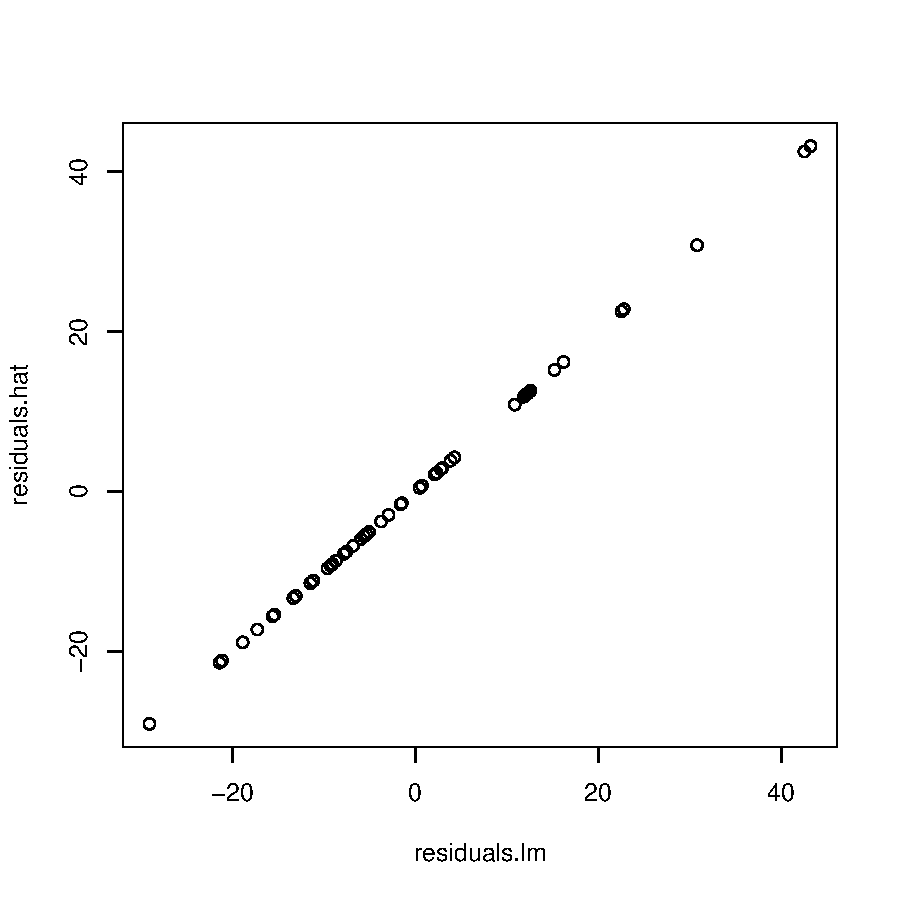
\includegraphics{HW5-003}
\end{figure}

\item $\hat{\sigma^2}$ is calculated as
\begin{Schunk}
\begin{Sinput}
> # calculating estimated variance
> n<-length(distance)
> p<-2
> var.hat<-(1/(n-p))*(t(residuals.hat)%*%(residuals.hat))
> var.hat
\end{Sinput}
\begin{Soutput}
         [,1]
[1,] 236.5317
\end{Soutput}
\end{Schunk}

\item $\hat{y}$ are calculated as
\begin{figure}[H]
\begin{Schunk}
\begin{Sinput}
> # calculating Hat Matrix
> Hat.mat<-X%*%(solve(t(X)%*%X))%*%(t(X))
> # calculated estimated response
> y.hat<-Hat.mat%*%distance
> # estimated response from lm
> y.hat.lm<-fit$fitted.values
> # plotting y.hat vs. y.hat.lm
> plot(y.hat.lm,y.hat)
\end{Sinput}
\end{Schunk}
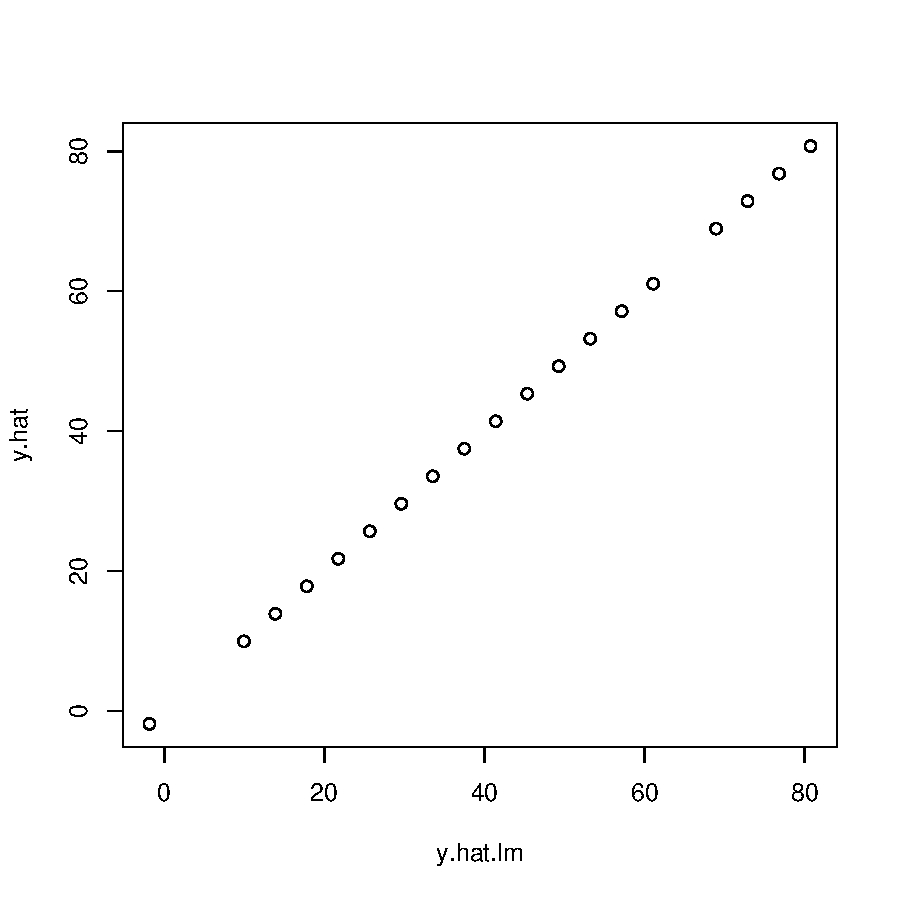
\includegraphics{HW5-005}
\end{figure}
\clearpage

\item $\text{se}_k$ for the parameters are calculated as
\begin{Schunk}
\begin{Sinput}
> # calculating variance of estimated parameters
> sqrt.beta.var.hat<-rep(0,2)
> L<-(solve(t(X)%*%X))
> for (i in 1:2){
+   sqrt.beta.var.hat[i]<-sqrt(var.hat*L[i,i])
+ }
> sqrt.beta.var.hat
\end{Sinput}
\begin{Soutput}
[1] 6.7584402 0.4155128
\end{Soutput}
\end{Schunk}

\item The p-values are calculated as:
\begin{Schunk}
\begin{Sinput}
> # calculating p-values
> p.values<-rep(0,2)
> for (i in 1:2){
+   p.values[i]<-2*pt((-abs(beta.hat[i])/sqrt.beta.var.hat[i]), df=n-p)
+ }
> p.values
\end{Sinput}
\begin{Soutput}
[1] 1.231882e-02 1.489836e-12
\end{Soutput}
\end{Schunk}

\item The coefficient of determination can be calculated as:
\begin{Schunk}
\begin{Sinput}
> R.sq<-(t(y.hat-mean(y.hat))%*%(y.hat-mean(y.hat)))/(t(distance-mean(distance))%*%(distance-mean(distance)))
> R.sq
\end{Sinput}
\begin{Soutput}
          [,1]
[1,] 0.6510794
\end{Soutput}
\end{Schunk}
\en
\end{document}
